\section{Approach and Uniqueness}

% In our work, three approaches are essential to build a natural language based shell command synthesizer that is practically useful. 
Our approach consists of three parts. First, we hire part-time programmers to collect shell commands and their natural language descriptions from the massive amount of shell-scripting tutorials and forums online, which results in a dataset that is orders of magnitude larger than those in previous works. Second, we restrict the domain to only commonly used file system operations to dramatically narrow the search space. We measure the ``commonness" based on the statistics of shell commands occurred in the crowdsourcing data. Third, we make use of the state-of-the-art incremental parsing techniques in NLP to increasing the search efficiency~\cite{zhao2014type,dyer2015transition,huang2010dynamic}, which allows us to explore a richer semantic space much faster. This framework can be generalized to more scripting languages.

\subsection{Havesting the Training Examples}

We built a web application that allows users to search\footnote{Powered by Google Search API: \url{https://cse.google.com/}.} for web pages that contains commonly used file system shell commands and their corresponding English descriptions. Examples of such web pages include tutorials, tech blogs, question-answering forums and course materials (*.pdf, *.doc, *.txt, etc.). The users are then asked to browse each retrieved web page and select all pairs of shell commands and their natural language descriptions found on the web page. We restrict the shell commands to be one-liners and the natural language description to be a single sentence. For the most commonly used commands, the natural language description can usually be copied verbatim from the web pages. The rest of the cases require the user to come up with their own descriptions using their background knowledge and the information on the web page. The users in our study are freelancers who are familiar with shell scripting. % hired using Upwork\footnote{\url{https://www.upwork.com/}}. 
The first two freelancers we hired collect 70 and 71 pairs respectively, over a 2-hour window. 

\subsection{Pruning the Search Space}

Since almost any operation performed by the operating system can be written in a shell script, it is important to select a subset of functionality to cover as a first step. 
In this work, we specifically look at file system operations. We restrict the first token of the command to be {\tt find}, but allow pipe structures that redirect the output of a {\tt find} command to other commands. At first glance, this seems to drastically cut the search space. However, the problem still remains difficult, for the user may describe the set of files/directories (s)he is looking for using \emph{name}, \emph{type}, \emph{permission}, \emph{size}, \emph{access time} and more. Extracting those attributes from the natural language is challenging. Besides, solving the ``find" problem is specifically valuable, for it gives us a filter on the files, and more functionality may be implemented by redirecting the filter output to other commands.
% since many requests can be accomplished using {\tt find} even if they are not explicitly searching for anything. Examples of such queries include \textit{sort files by size in the current directory} and \textit{check if my file has 644 permission}.   such as \textit{removing files older than 30 days},
% The ``commonness" is 
We hope that the training set we gathered automatically reflects the popularity of attributes users tend to specify, and hence the frequently occurred ones can be well learnt\footnote{It is possible that people tend to not post certain commands due to complexity and other reasons and we end up getting a biased training set. It this turned out to be the case, we will develop methods to compensate for the bias.}.

To make the trained model more generalizable, we normalize the command arguments by replacing the attribute values with their semantic types, 
% \footnote{Argument normalization may not be necessary if we decide to use neural network based models, for the models can automatically assign similar representations to arguments of the same type.}, 
as shown in figure~\ref{fig:norm}. The types are derived semi-automatically using man-pages.

\begin{figure}[t]
    \centering
    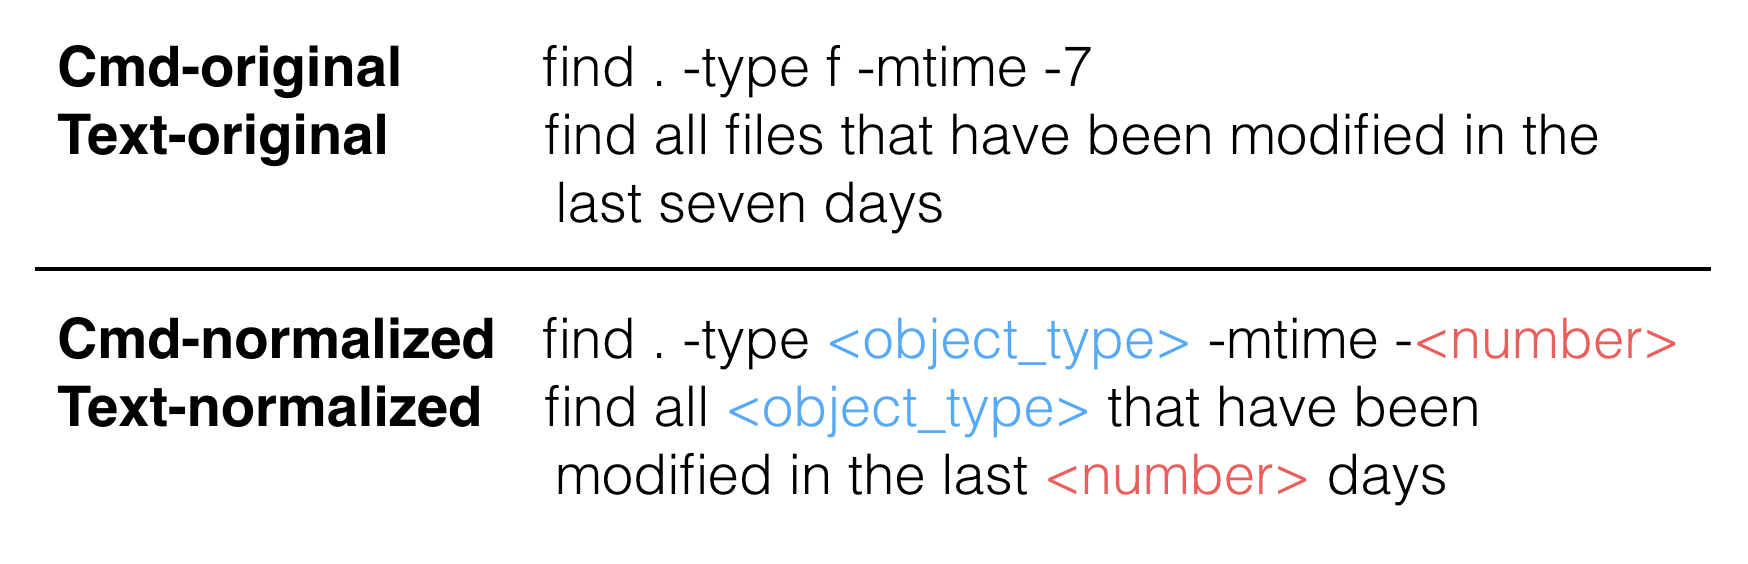
\includegraphics[width=3.3in]{normalization}
    \caption{Normalizing command arguments and the corresponding English noun phrases.}
    \label{fig:norm}
\end{figure}

\subsection{Incremental Parsing and Synthesis}

Most existing PBNL framework adopted a top-down approach that enumerates all legal programs according to the grammar of the programming language, and use the natural language to guide the enumeration~\cite{DBLP:journals/corr/DesaiGHJKMRR15,bashsynthesis}. For example,~\cite{bashsynthesis} applied top-down beam search with simple token based scoring. For head commands with a large set of options such as {\tt find}, enumerating all possible commands up to length 5 takes about 3s for a small beam size of 7, indicating the need for more aggressive pruning.

In this work, we plan to take a different approach that synthesizes the command bottom-up. The idea is based on the observation that the order of the shell command options is exchangable; therefore most of the time there exists a correct command whose options are in the same order as their corresponding natural language components\footnote{However, this assumption may be broken for commands with the ``pipe" structure. Noticed that in table~\ref{table:examples}, the first and the third command has options in the same order as their natural language correspondences. The second command exactly reversed the order in the natural language specification, and it contains one ``pipe"}. Inspired by existing work on shift-reduce natural language parsing~\cite{zhao2014type,dyer2015transition,huang2010dynamic}, we will train a synthesizer that parses the natural language incrementally, and maps the parsed natural language components into partial shell commands on the fly. % This process is illustrated in figure~\ref{}.